% Uncomment this to make slides with overlays:
\documentclass[slides]{beamer}

% Uncomment these (but comment the above \documentclass line) to make handouts:
%\documentclass[handout]{beamer}
%\usepackage{pgfpages}
%\pgfpagesuselayout{2 on 1}[border shrink=5mm]
%\pgfpageslogicalpageoptions{1}{border code=\pgfusepath{stroke}}
%\pgfpageslogicalpageoptions{2}{border code=\pgfusepath{stroke}}

\usepackage[]{graphicx, color, hyperref}

\mode<presentation>
{
	%\usetheme[secheader]{Boadilla}
	%\usecolortheme[rgb={.835, .102,.169}]{structure}  
	\usetheme[width= 0cm]{Goettingen}
	%\setbeamercovered{transparent}
}
\setbeamertemplate{navigation symbols}{}
\setbeamertemplate{footline}[frame number]

\definecolor{blue2}{rgb}{0.278,0.278,0.729} 
\newcommand{\blue}[1]{\textcolor{blue2}{#1}}
\newcommand{\white}[1]{\textcolor{white}{#1}}
\newcommand{\red}[1]{\textcolor{red}{#1}}
\newcommand{\xbar}{\overline{x}}
\newcommand{\ybar}{\overline{y}}
\newcommand{\phat}{\widehat{p}}
\newcommand{\prob}{\mbox{Pr}}
\newcommand{\E}{\mathbb{E}}
\newcommand{\Var}{\mbox{Var}}
\newcommand{\cp}{\oplus}
\newcommand{\cm}{\circleddash}


\title{Lecture 1: Laying the Foundations + Terminology}
\author{Chapters 1.1-1.2}
\date{}


\begin{document}
%------------------------------------------------------------------------------
\begin{frame}
\titlepage
\end{frame}
%------------------------------------------------------------------------------


%------------------------------------------------------------------------------
\begin{frame}
\frametitle{Goals for Today}
\begin{itemize}
  \item Go over the syllabus 
  \item Show some fun examples 
  \item Discuss how to evaluate the efficacy of a \blue{treatment}
  \item Describe the different kinds of \blue{variables} we'll consider
\end{itemize}

\end{frame}
%------------------------------------------------------------------------------


%------------------------------------------------------------------------------
\begin{frame}
\frametitle{What is statistics?}

(Direct from text) The general scientific process of investigation can be summed up as follows:

\begin{enumerate}
\pause\item Identify the scientific question or problem
\pause\item Collect relevant data on the topic
\pause\item Analyze the data
\pause\item Form a conclusion \pause and \blue{communicate it}
\end{enumerate}

\pause Statistics concerns itself with points 2 through 4.

\end{frame}
%------------------------------------------------------------------------------


%------------------------------------------------------------------------------
\begin{frame}[fragile]
\frametitle{Your Majors}
\begin{small}
\begin{verbatim}
                      Biology                     Economics 
                           11                             5 
                      History         Environmental Studies 
                            4                             3 
                  Mathematics                    Psychology 
                            3                             3 
Biochem and Molecular Biology                     Chemistry 
                            2                             2 
 International Policy Studies                   Linguistics 
                            2                             2 
                    Undecided                  Anthropology 
                            2                             1 
        Economics/Mathematics    Environmental Studies-Hist 
                            1                             1 
Environmental Studies-Pol Sci                       Physics 
                            1                             1 
                    Sociology 
                            1 
\end{verbatim}
\end{small}
\end{frame}
%------------------------------------------------------------------------------


%------------------------------------------------------------------------------
\begin{frame}[fragile]
\frametitle{Example: 2012 Election - Nate Silver's Predictions vs Actual Results}
\begin{center}
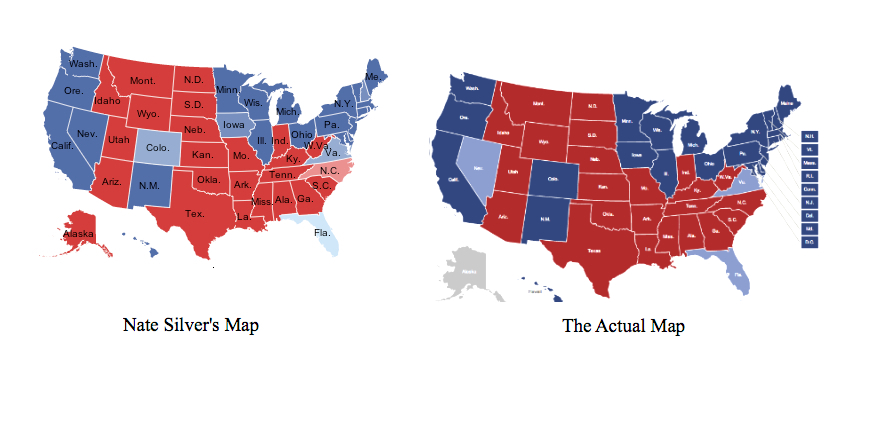
\includegraphics[width=\textwidth]{figure/nate_silver.jpg}
\end{center}
\begin{center}
\end{center}
\end{frame}
%------------------------------------------------------------------------------


%------------------------------------------------------------------------------
\begin{frame}[fragile]
\frametitle{Example: Brain \& Breast Cancer in Western Washington}

My PhD dissertation involved detecting cancer ``clusters'': areas of residual spatial variation of disease risk.

\vspace{1cm}

We modeled the (Bayesian) probability of cluster membership for each of the $n=887$ census tracts in Western Washington in 2000, using cancer data from 1995--2005, controlling for age, race, and gender.  




\end{frame}
%------------------------------------------------------------------------------


%------------------------------------------------------------------------------
\begin{frame}[fragile]
\frametitle{Brain Cancer Controlling for Age, Race, \& Gender}
\begin{center}
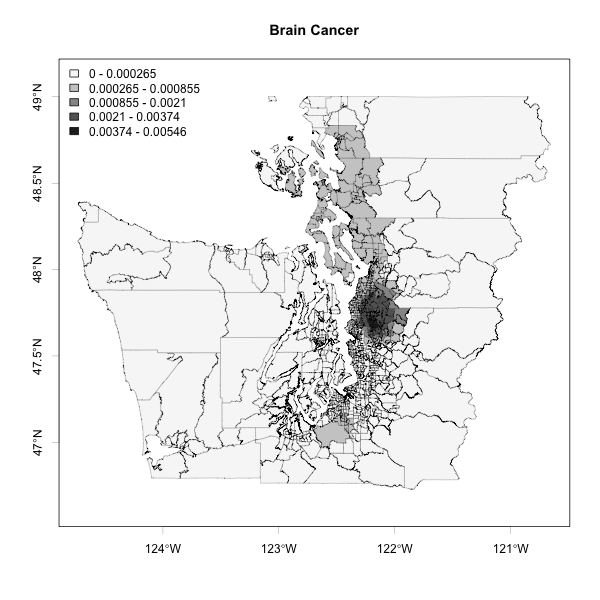
\includegraphics[width=8.5cm]{figure/brain.png}
\end{center}
\end{frame}
%------------------------------------------------------------------------------


%------------------------------------------------------------------------------
\begin{frame}[fragile]
\frametitle{Breast Cancer Controlling for Age, Race, \& Gender}
\begin{center}
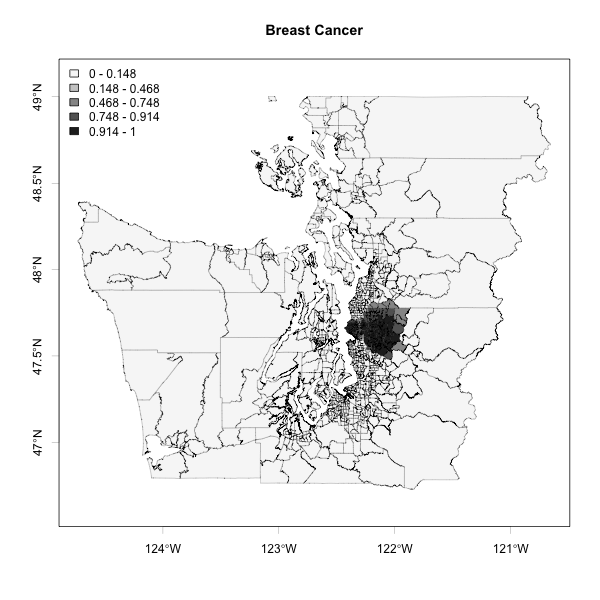
\includegraphics[width=8.5cm]{figure/breast.png}
\end{center}
\end{frame}
%------------------------------------------------------------------------------


%------------------------------------------------------------------------------
\begin{frame}[fragile]
\frametitle{Income per Capita Quintiles}
\begin{center}
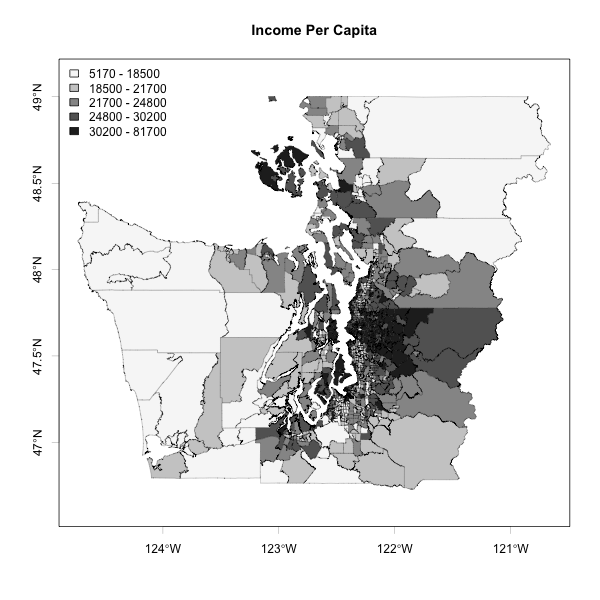
\includegraphics[width=8.5cm]{figure/income.png}
\end{center}
\end{frame}
%------------------------------------------------------------------------------


%------------------------------------------------------------------------------
\begin{frame}[fragile]
\frametitle{Breast Cancer Adjusted for Income as Well}
\begin{center}
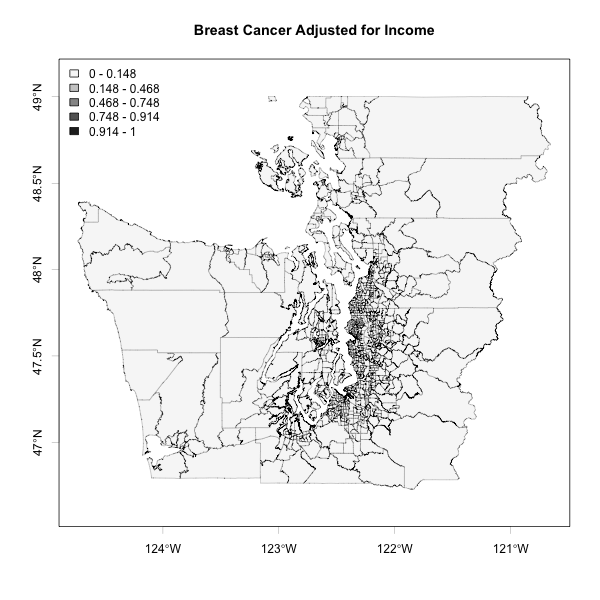
\includegraphics[width=8.5cm]{figure/breast_new.png}
\end{center}
\end{frame}
%------------------------------------------------------------------------------


%------------------------------------------------------------------------------
\begin{frame}[fragile]
\frametitle{Example: Social Network Display of a Recent Party I Had}
\begin{center}
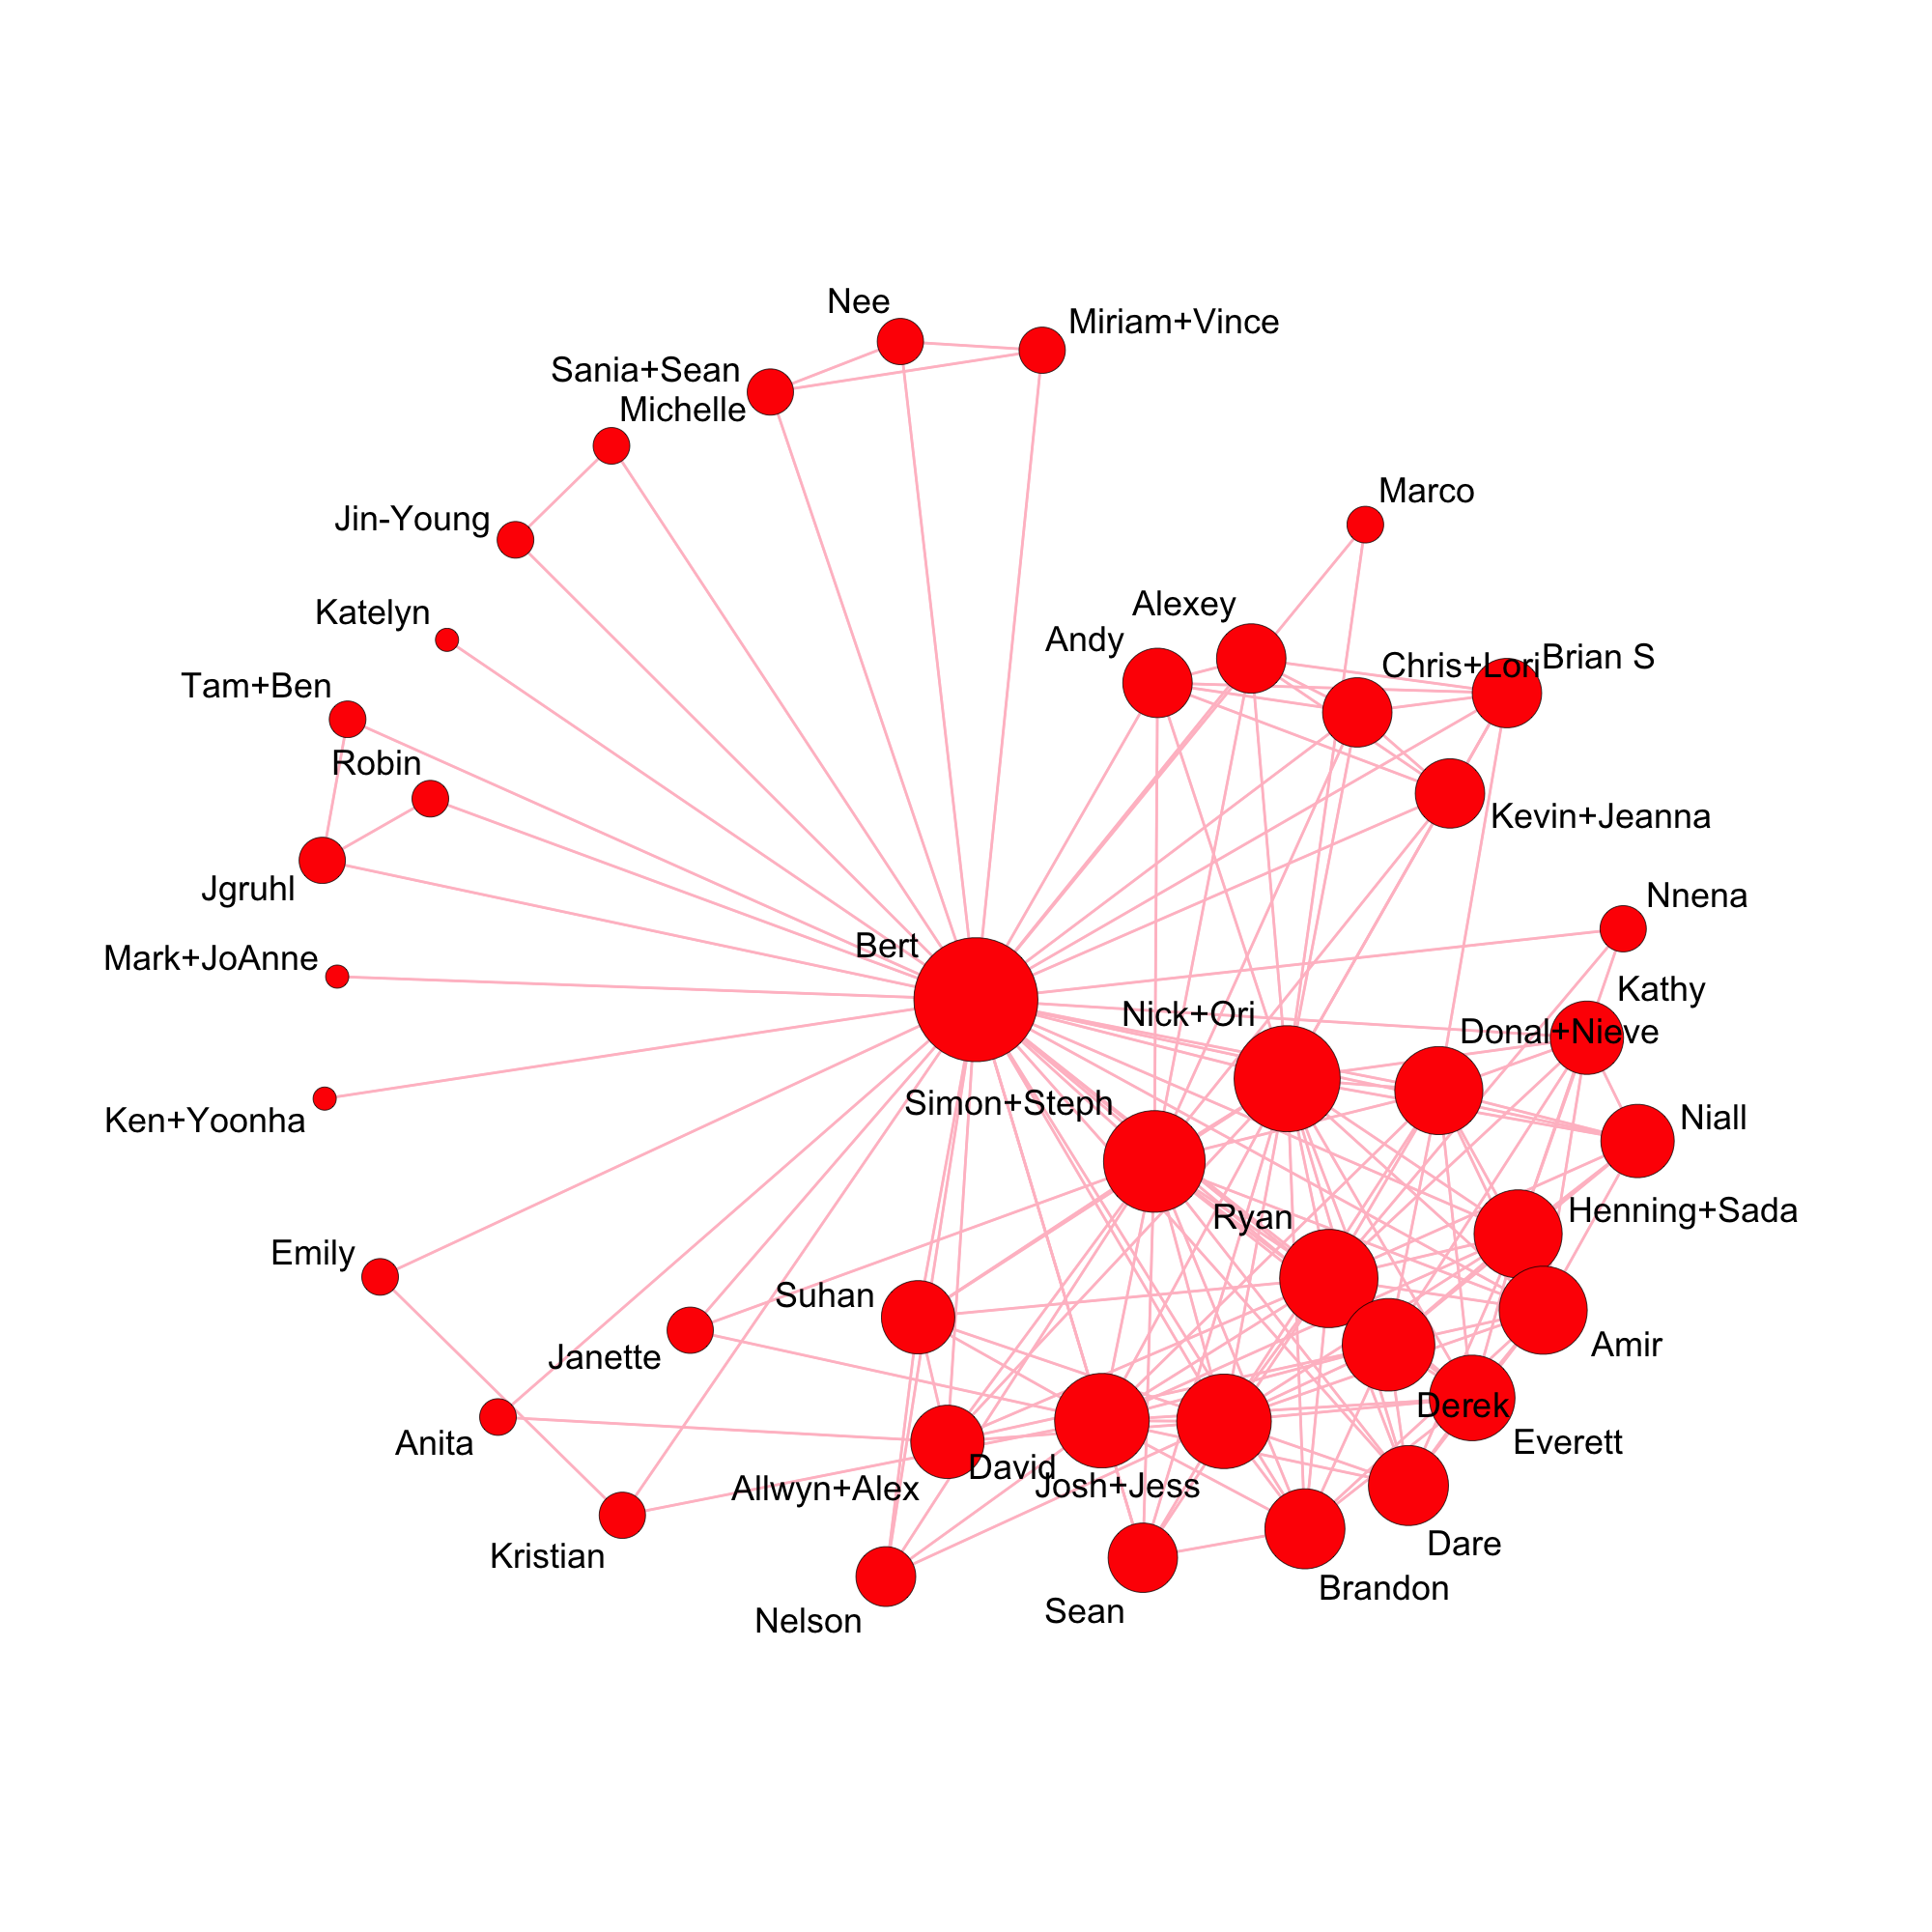
\includegraphics[width=8cm]{figure/network.png}
\end{center}
\end{frame}
%------------------------------------------------------------------------------


%------------------------------------------------------------------------------
\begin{frame}
\frametitle{Say we want answer the following questions:}
\begin{itemize}
\pause\item Does a new kind of cognitive therapy alter levels of depression in patients?
\pause\item Or you question the effectiveness of antioxidants in preventing cancer.
\pause\item Will reassuring potential new users to a gambling website that we won't spam them increase the sign-up rate?
\end{itemize}

\end{frame}
%------------------------------------------------------------------------------



%------------------------------------------------------------------------------
\begin{frame}
\frametitle{Evaluating the efficacy of a `treatment'}
In all the above cases, you are questioning the efficacy of a \blue{treatment/intervention}.  One way to evaluate the efficacy is via an \blue{experiment} where you define
\begin{itemize}
\pause\item A \blue{control} group: the ``business as usual'' baseline group
\pause\item A \blue{treatment} group:  the group that receives/is subject to the treatment/intervention
\end{itemize}
\pause and make comparisons.

\end{frame}
%------------------------------------------------------------------------------



%------------------------------------------------------------------------------
\begin{frame}
\frametitle{Website Experiments}
\begin{center}
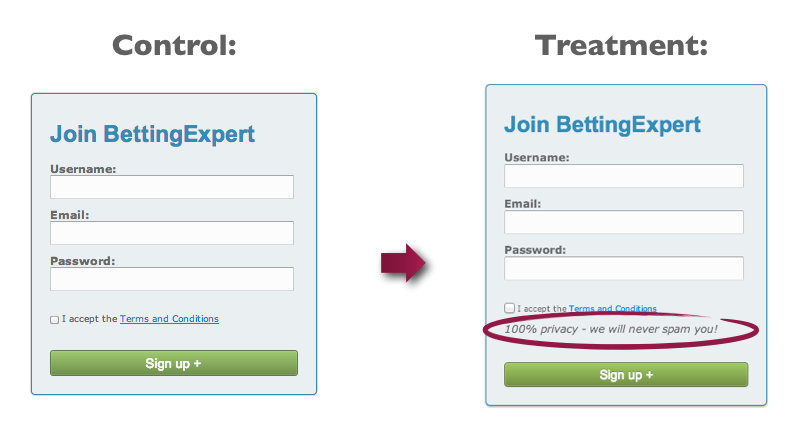
\includegraphics[width=9cm]{figure/control_treatment.png}
\end{center}
\end{frame}
%------------------------------------------------------------------------------



%------------------------------------------------------------------------------
\begin{frame}
\frametitle{Example of a treatment vs control}
Two other examples in the media of late
\begin{itemize}
\item Facebook's tinkering with user's emotions \blue{\href{http://www.nytimes.com/2014/06/30/technology/facebook-tinkers-with-users-emotions-in-news-feed-experiment-stirring-outcry.html}{(link)}}
\item OkCupid's admission that they experiment on human beings \blue{\href{http://blog.okcupid.com/index.php/we-experiment-on-human-beings/}{(link)}}
\end{itemize}

\end{frame}
%------------------------------------------------------------------------------



%------------------------------------------------------------------------------
\begin{frame}[fragile]
\frametitle{Variables}
A \blue{variable} is a description of any characteristic whose value may change from one unit in the population to the next:
%\begin{center}
%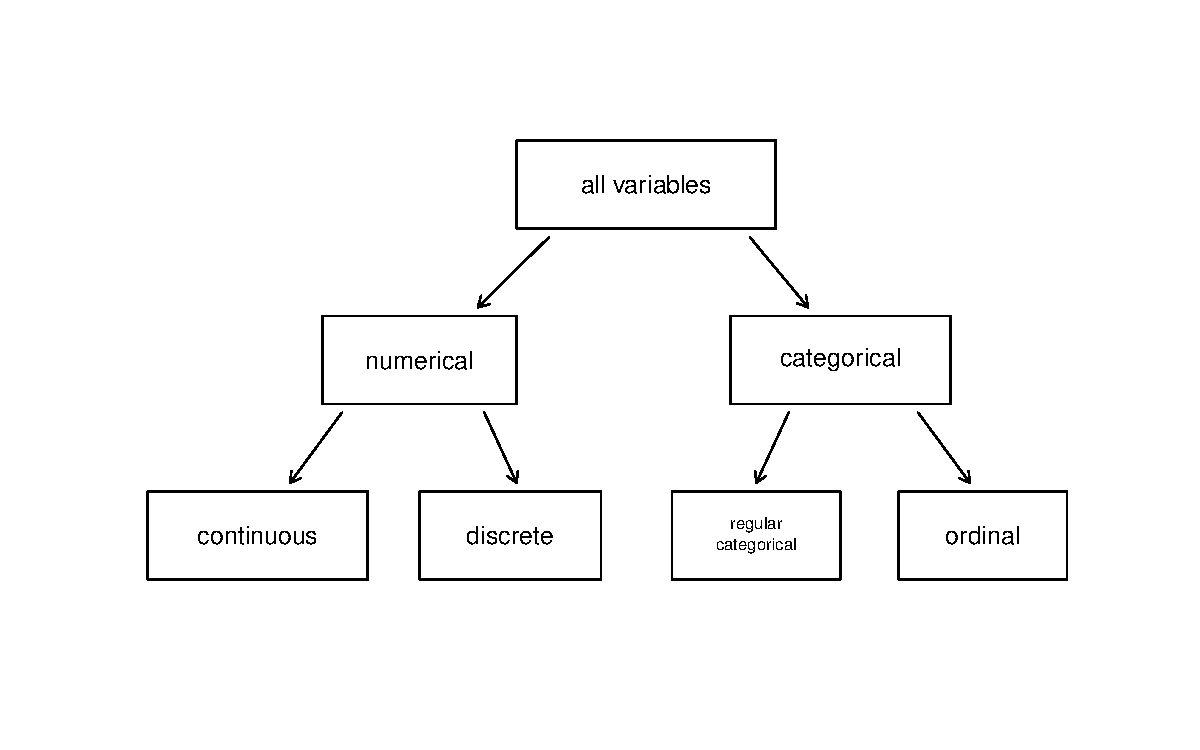
\includegraphics[width=\linewidth]{figure/flow-chart} 
%\end{center}
\vspace{3in}

\end{frame}
%------------------------------------------------------------------------------



%%------------------------------------------------------------------------------
%\begin{frame}
%\frametitle{Variables}
%A \blue{variable} is a description of any characteristic whose value may change from one unit in the population to the next:
%\begin{enumerate}
%\pause\item gender of an engineer:  \blue{categorical} variable
%\pause\item level of education (high school/GED, college, grad school): \blue{ordinal} variable
%\pause\item number of major defects on a newly manufactured phone: \blue{discrete} variable i.e. something you can count
%\pause\item temperature of the battery in a phone after 1 hour of use: \blue{continuous} variable; its possible values consist of an interval on the number line
%\end{enumerate}
%
%\end{frame}
%%------------------------------------------------------------------------------



%------------------------------------------------------------------------------
\begin{frame}
\frametitle{Data}

At its simplest, data are presented in a data table or matrix where (almost always) each
\begin{itemize}
\pause\item row corresponds to \blue{cases} or \blue{units of observation/analysis}
\pause\item column represents the variables corresponding to a particular observation
\end{itemize}

\pause It is almost always the case that 

\begin{itemize}
  \pause\item $n$ is the number of observations
  \pause\item $p$ is the number of variables
\end{itemize}

\end{frame}
%------------------------------------------------------------------------------




%------------------------------------------------------------------------------
\begin{frame}[fragile]
\frametitle{Data Summaries}

Consider the variable "federal spending per capita" in each of the 3,143 counties in the US.  One can hardly digest this:

\begin{tiny}
\begin{verbatim}
   [1]   6.068095   6.139862   8.752158   7.122016   5.130910   9.973062   9.311835  15.439218
   [9]   8.613707   7.104621   6.324061  10.640378   9.781442   8.982702   6.840035  20.330684
  [17]   9.687698  11.080738   7.839761   9.461856   9.650295   7.760627  25.774791  13.948106
   ...
[3121]   7.520731  10.246400   3.106800  17.679572   4.824044   7.247212   8.484211   8.794626
[3129]   9.829593   8.100945  17.090715   4.855849   6.621378  22.587359  10.813260  11.422522
[3137]   9.580265   4.368986   5.062138   6.236968   4.549105   8.713817   6.694784
\end{verbatim}
\end{tiny}

\end{frame}
%------------------------------------------------------------------------------




%------------------------------------------------------------------------------
\begin{frame}[fragile]
\frametitle{Data Summaries}
We can't interpret all the data at once; we need to boil it down via \blue{summary statistics}, single numbers summarizing a large amount of data.

\vspace{0.5cm}

\pause Using the \verb#summary()# command in \verb#R#:

\begin{small}
\begin{verbatim}
   Min. 1st Qu.  Median    Mean 3rd Qu.    Max.    NA's 
  0.000   6.964   8.669   9.991  10.860 204.600       4 
\end{verbatim}
\end{small}


\end{frame}
%------------------------------------------------------------------------------


%------------------------------------------------------------------------------
\begin{frame}[fragile]
\frametitle{Relationships between variables}
We can best display the relationship between two variables using a \blue{scatterplot AKA bivariate plot}:

\begin{center}
\pause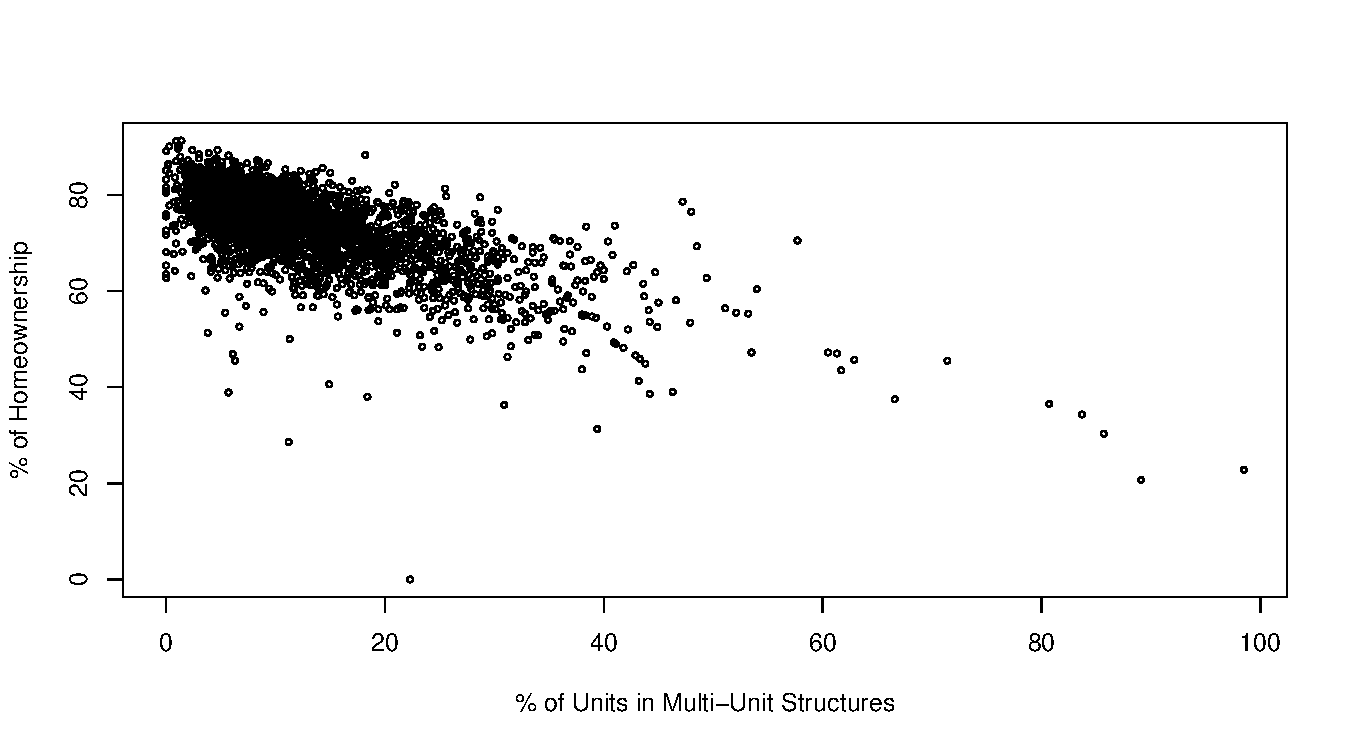
\includegraphics[width=\linewidth]{figure/relationships} 
\end{center}

\end{frame}
%------------------------------------------------------------------------------


%------------------------------------------------------------------------------
\begin{frame}
\frametitle{Relationships between variables}
Almost always we are interested in the relationship between two or more variables.

\vspace{0.25cm}

\pause A pair of variables are either related in some way (\blue{associated}) or not (\blue{independent}).  No pair of variables are both associated and independent.   

\vspace{0.25cm}

\pause We can have either a \blue{negative association} (as the value of one variable increases, the other decreases) or a \blue{positive association}.

\end{frame}
%------------------------------------------------------------------------------


%------------------------------------------------------------------------------
\begin{frame}[fragile]
\frametitle{Relationships between variables}
We can consider a third variable in the previous plot.
\begin{center}
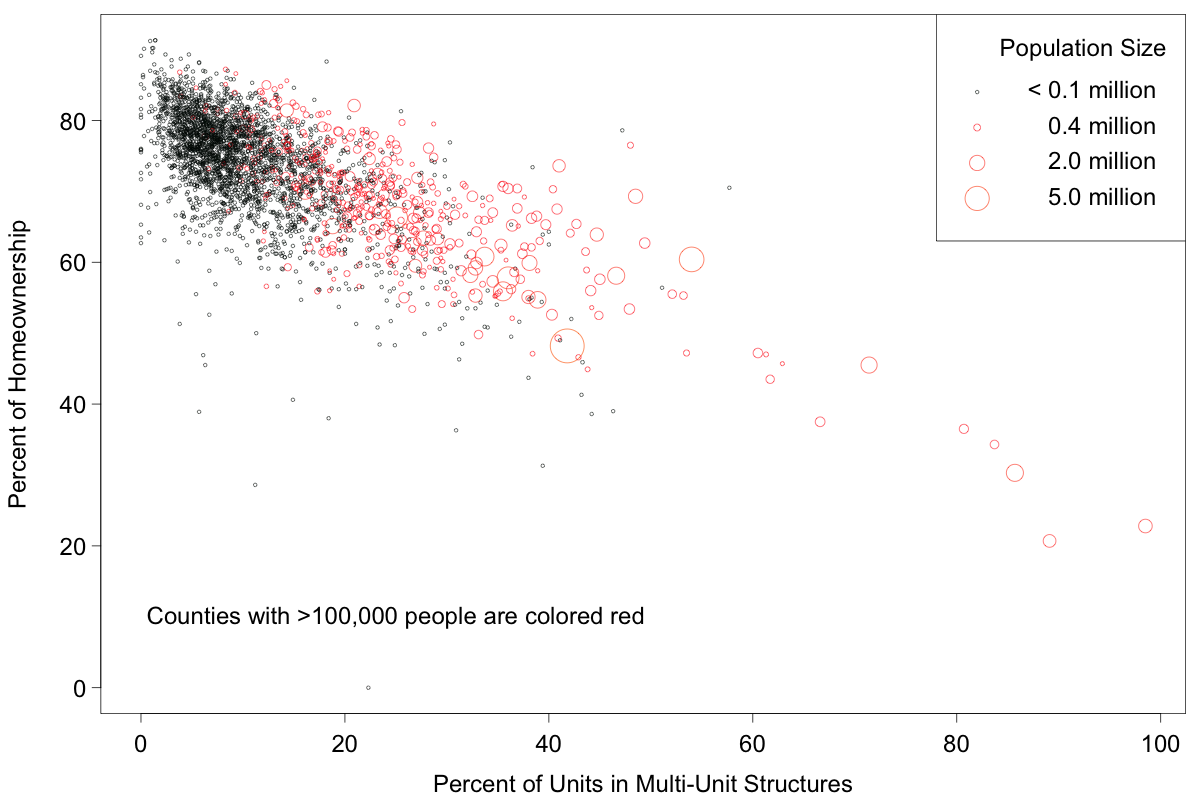
\includegraphics[width=\textwidth]{figure/MHP.png}
\end{center}
\end{frame}
%------------------------------------------------------------------------------





\end{document}









